\documentclass[]{scrartcl}
\usepackage{inputenc}
\usepackage[german]{babel}
\usepackage[colorlinks=true,urlcolor=blue]{hyperref}
\usepackage{amsmath}
\usepackage{amsfonts}
\usepackage{graphicx}

%opening
\title{Mathematische Knobeleien}
\subtitle{Teil 3 -- Ein Dreieck im Trapez}
\author{Mathematik - Verständlich gemacht!\footnote{Email: \href{mailto:kontakt@mschulte-mathematik.ruhr}{kontakt@mschulte-mathematik.ruhr}}}

\begin{document}

\maketitle

\section*{Problemstellung}
Es sei $T:=ABCD$ ein gleichschenkliges Trapez mit den 
Seiten\footnote{Wir identifizieren Seitennamen mit ihren 
Längen.} $a:=AB$, $b:=BC$, $c:=CD$ und $d:=DA$. Seine Höhe
bezeichnen wir mit $h_T$. Nun ziehen wir die
beiden Diagonalen $AC$ und $DB$ ein und bezeichnen ihren 
Schnittpunkt mit $S$. Von $C$ und $D$ fällen wir jeweils das
Lot auf $a$; die entstehenden Schnittpunkte nennen wir $S_C$ bzw.
$S_D$. Es entsteht ein Dreieck $\Delta := S_DS_CS$. 
Bestimme den Flächeninhalt von $\Delta$.

\section*{Lösung}
Wir kombinieren Methoden der klassischen Geometrie und der 
analytischen Geometrie. Im Folgenden verwenden wir die 
Bezeichnungen der nachstehenden Skizze.

\noindent 
\begin{figure}[h]
	\centering
	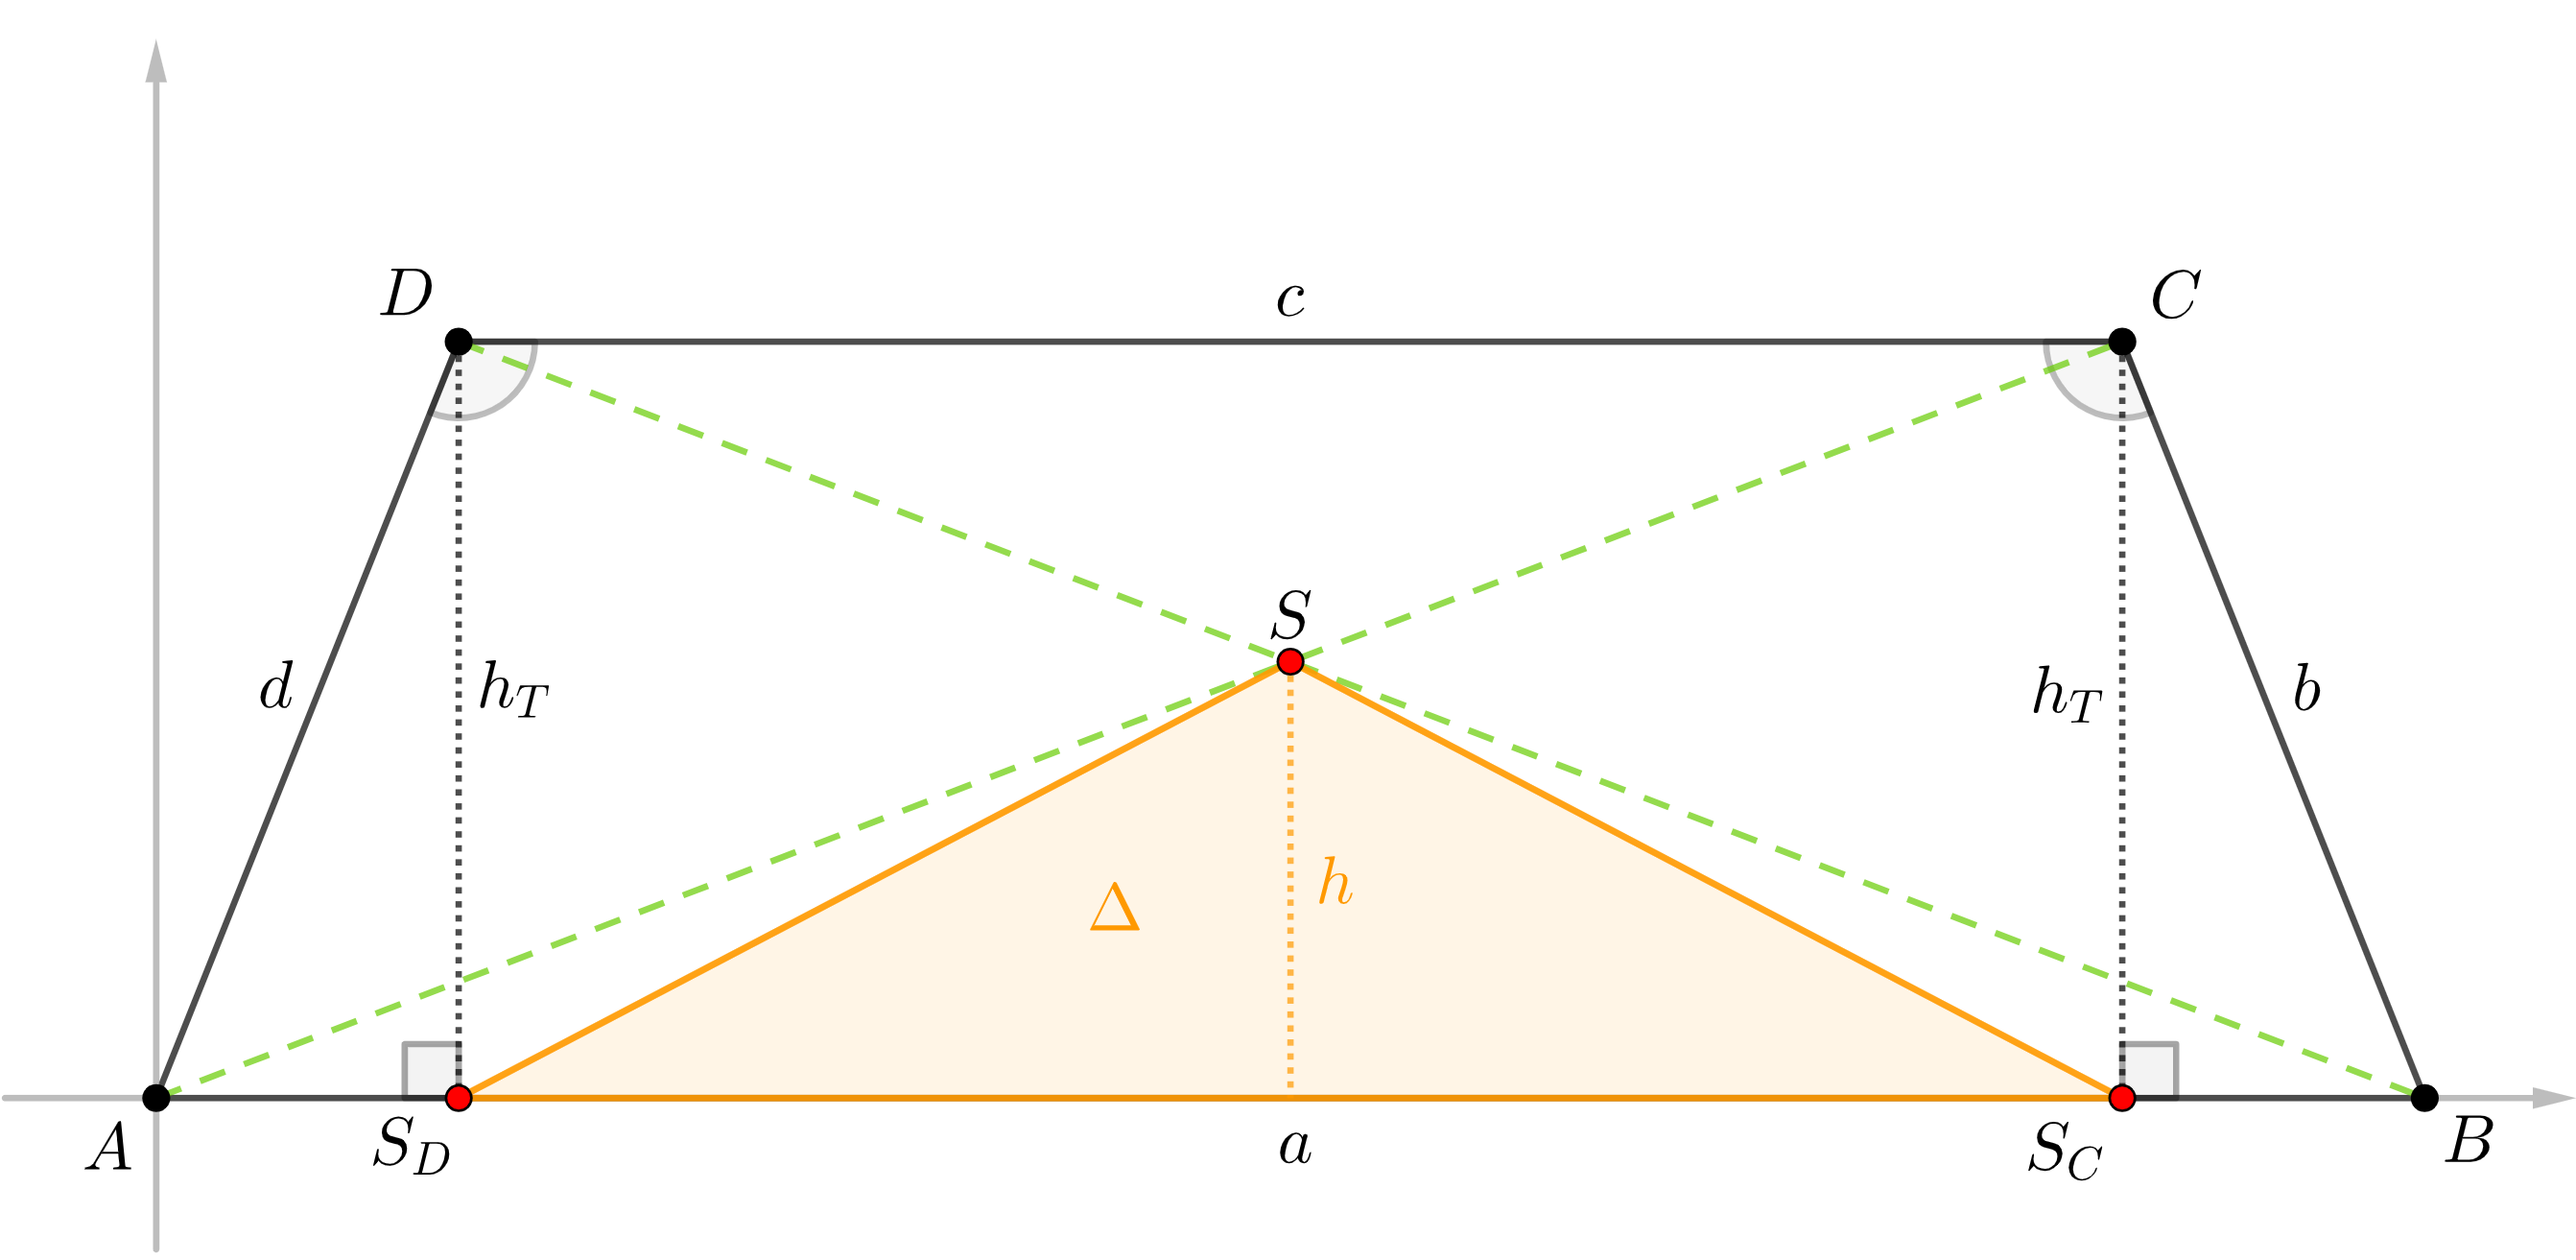
\includegraphics[width=10cm]{abbildungen/MaKno_3_Figur_1.png}
	\label{fig:1}
\end{figure}

\noindent 
Zudem setzen wir $t_1 := AS_D$, $t_2 := AS_C$, $t_3 := S_CB$ und 
$t_4 := S_DS_C$.

\noindent 
Da $T$ gleichschenklig ist, ist $b=d$ und folglich $t_1=t_3$.
Aus dem Satz von Pythagoras folgt 
$$
t_1 = \sqrt{d^2-h_T^2} = t_3.
$$
Daraus ergeben sich unmittelbar
$$
t_2 = a-t_3 = a-\sqrt{d^2-h_T^2} \text{ und } 
t_4 = a-t_1-t_3 = a-2\sqrt{d^2-h_T^2}.
$$
Nun führen wir ein kartesisches Koordinatensystem mit Ursprung in
$A$ ein, sodass $a$ auf der Abszissenachse liegt. Damit lesen wir
die Koordinaten von $A,B,C$ und $D$ ab:
$$
A = (0,0), ~ B = (a,0), ~ C = (t_2,h_T), ~ D = (t_1,h_T).
$$
Hiermit bestimmen wir Funktionsgleichungen für die Diagonalen:
\begin{align*}
d_1(x) &= \frac{h_T}{a-\sqrt{d^2-h_T^2}}x, ~ x \in [0,t_2] ~
\text{ (Diagonale $AC$)}
\\
d_2(x) &= \frac{h_t}{\sqrt{d^2-h_T^2} - a}x - \frac{a\cdot h_T}
{\sqrt{d^2-h_T^2}-a}, ~ x \in [t_1,a] ~ \text{ (Diagonale $DB$)}
\end{align*}
Gleichsetzen liefert den Schnittpunkt $S$ der beiden Diagonalen:
$$
S = \left ( \frac{a}{2}, \frac{a \cdot h_t}{a-\sqrt{d^2-h_T^2}}
 \right ).
$$
Es ist also $h = y(S)$. Hiermit erhalten wir den gesuchten 
Flächeninhalt als
$$
F_\Delta = \frac{1}{2} \cdot h \cdot t_4 =
\frac{1}{2} \cdot \frac{a \cdot h_T \cdot \left ( 
	a - 2\sqrt{d^2-h_T^2} \right )}{a- \sqrt{d^2-h_T^2}}.
$$

\section*{Ergänzungen}
Wir können den Flächeninhalt von $\Delta$ natürlich auch ausrechnen,
wenn $T$ nicht gleichschenklig ist; die Rechnungen werden lediglich
algebraisch \textit{komplizierter}, da wir keine Symmetrien mehr
ausnutzen können. Wir geben hier nur die Lösungen an, der Weg zur 
Herleitung läuft analog zu oben.

\noindent 
\begin{figure}[h]
	\centering
	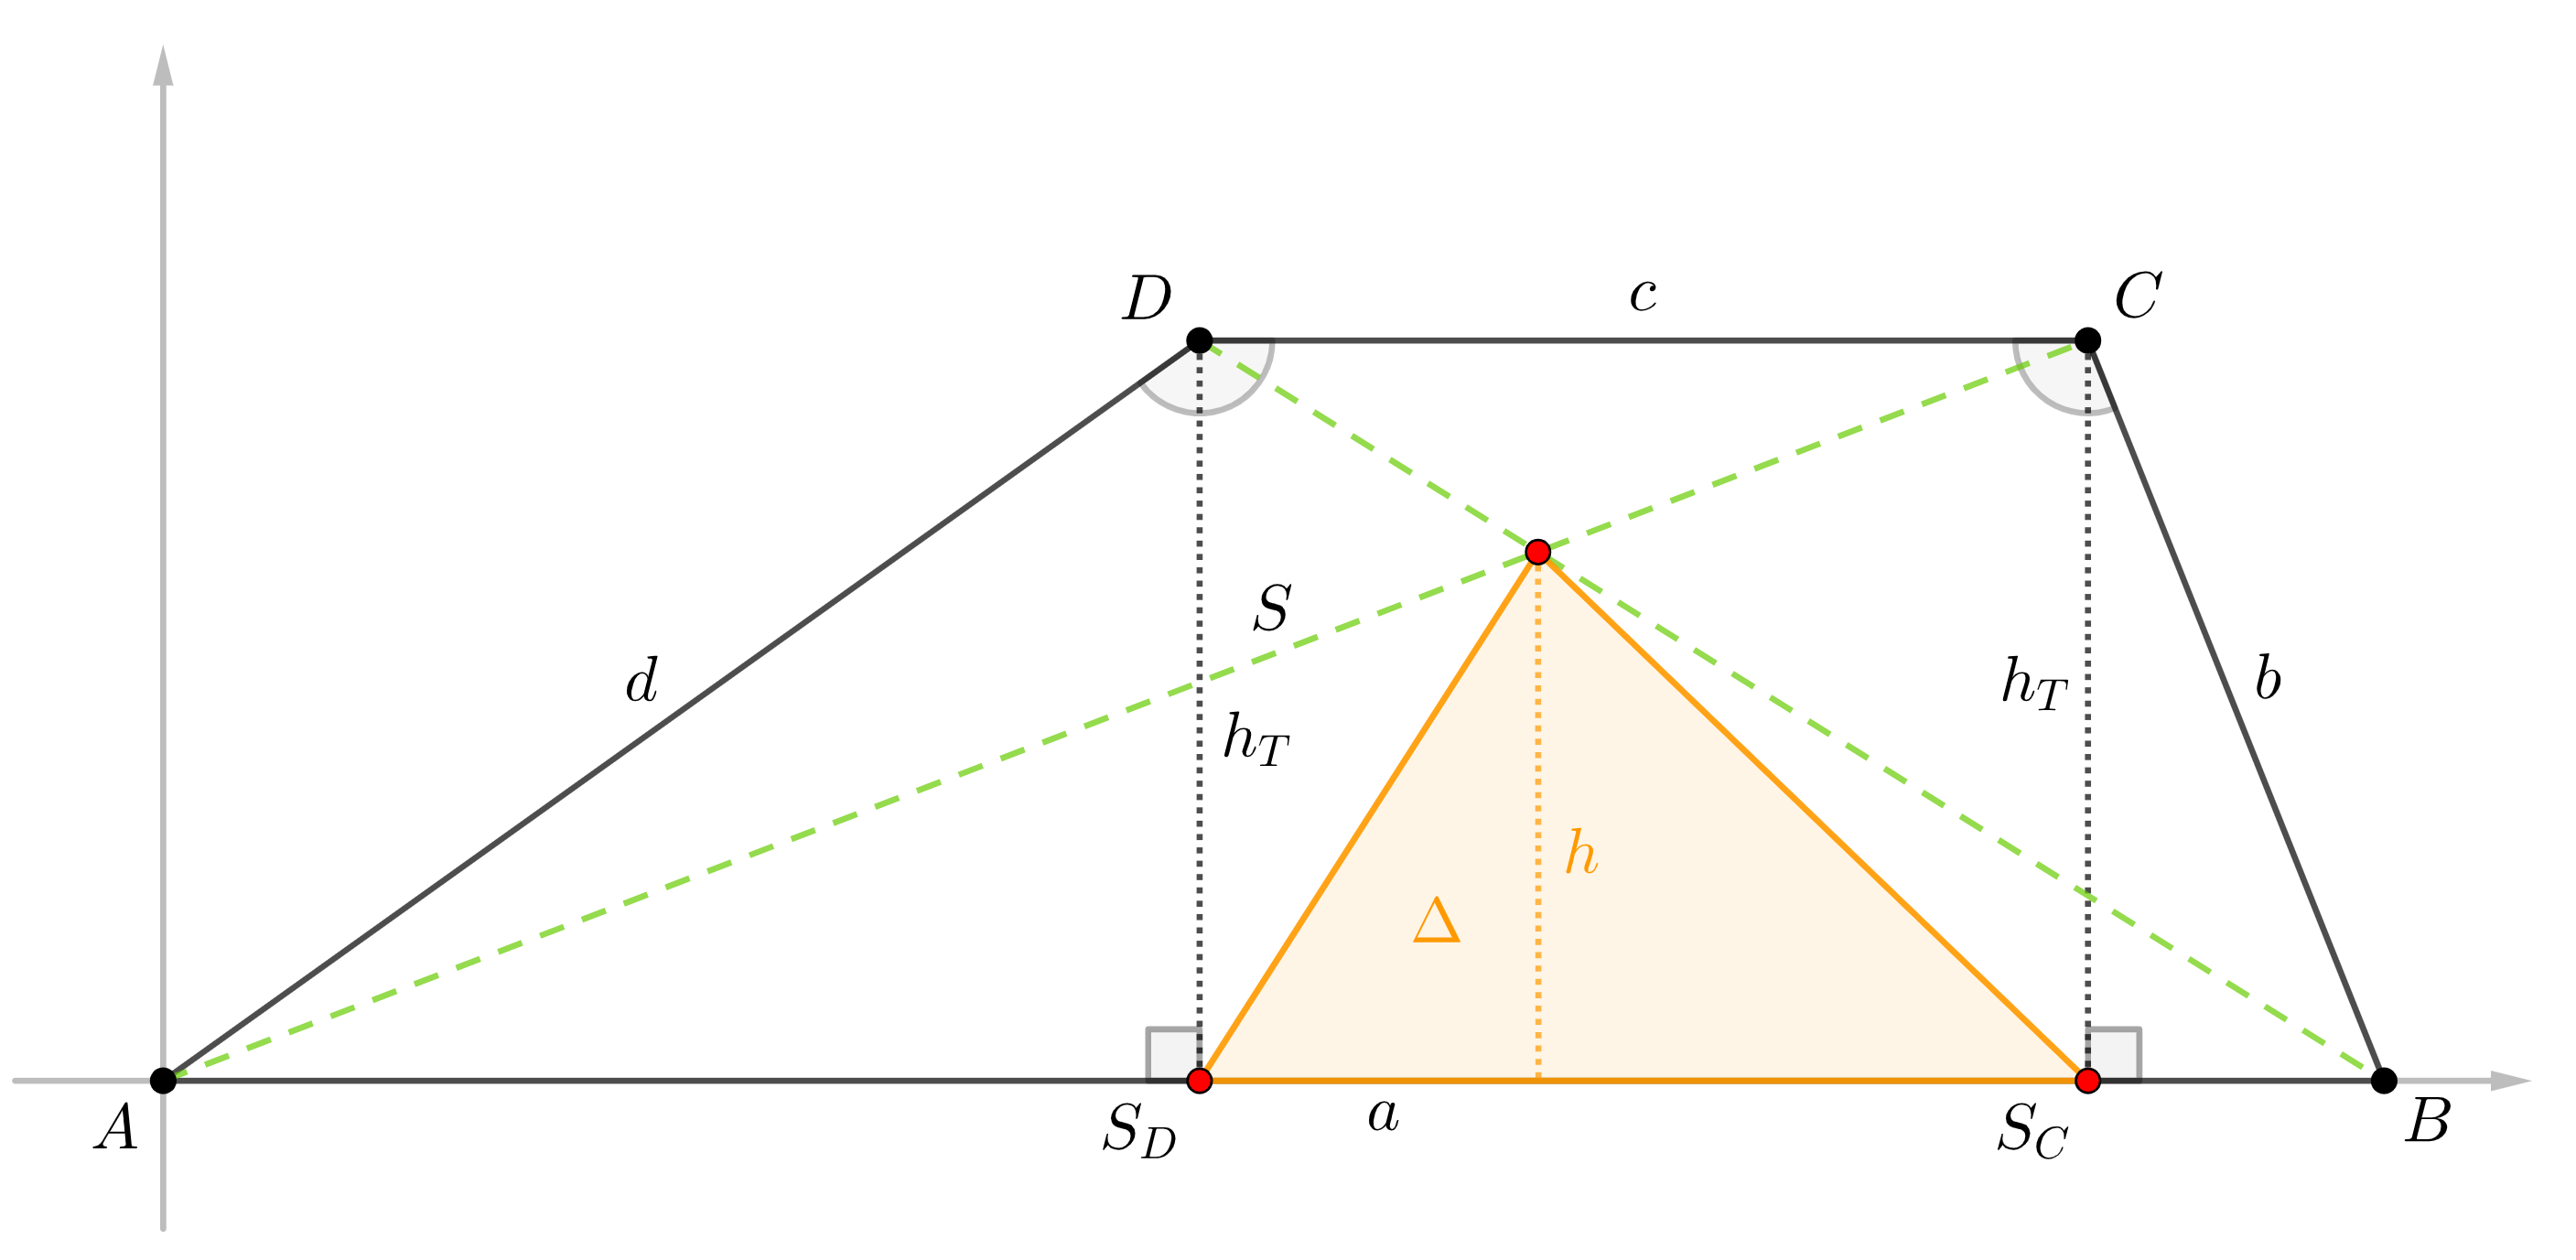
\includegraphics[width=10cm]{abbildungen/MaKno_3_Figur_2.png}
	\label{fig:2}
\end{figure}

\newpage

\noindent 
Die Bezeichnungen seien wie oben gewählt.

\noindent 
Punktkoordinaten:
$$
A = (0,0), ~ B = (a,0), ~ C = (t_2,h_T), ~ D = (t_1,h_T). 
$$
Diagonalengleichungen:
\begin{align*}
	d_1(x) &= \frac{h_T}{a-\sqrt{b^2-h_T^2}}x, ~ x \in [0,t_2] ~
	\text{ (Diagonale $AC$)}
	\\
	d_2(x) &= -\frac{h_t}{a-\sqrt{d^2-h_T^2}}x + \frac{a\cdot h_T}
	{a-\sqrt{d^2-h_T^2}}, ~ x \in [t_1,a] ~ \text{ (Diagonale $DB$)}
\end{align*}
Schnittpunkt:
\begin{align*}
	& d_1(x_S) = d_2(x_S)
	\\
	\Leftrightarrow & 
	\left ( 
		\frac{h_T}{a-\sqrt{b^2-h_T^2}} + 
		\frac{h_T}{a-\sqrt{d^2-h_T^2}}
	\right ) 
	x_S = \frac{a\cdot h_T}{a-\sqrt{d^2-h_T^2}}
	\\
	\Leftrightarrow & 
	\left ( 
		\frac{a-\sqrt{d^2-h_T^2}}{a-\sqrt{b^2-h_T^2}} + 1
	\right )
	x_S = a. ~ \text{ (Kürzen und Bruch rausmultiplizieren)}
\end{align*}
Setzen wir nun 
$$
	\frac{a-\sqrt{d^2-h_T^2}}{a-\sqrt{b^2-h_T^2}} + 1 =: \frac{1}{\Gamma},
$$
so erhalten wir 
$$
x_S = \Gamma \cdot a.
$$
Dies ist mit den vorherigen Ergebnissen konsistent, denn $b=d$ 
ergibt $\Gamma = \frac{1}{2}$. 

\noindent 
Flächeninhalt:
\begin{align*}
	F_\Delta 
	&=
	\frac{1}{2} \cdot \Gamma \cdot a \cdot 
	\left ( 
	a - \sqrt{d^2-h_T^2} - \sqrt{b^2-h_T^2}
	\right )
	\\ &=
	\frac{1}{2} \cdot a \cdot 
	\left (
		a-\sqrt{b^2-h_T^2}
	\right )
	\cdot 
	\frac
	{
		a - \sqrt{d^2-h_T^2} - \sqrt{b^2-h_T^2}
	}
	{
		2a - \sqrt{d^2-h_T^2} - \sqrt{b^2-h_T^2}
	}.
\end{align*}


\section*{Quellen}
Die Aufgabe entspringt eigenen Überlegungen.

\end{document}
